\documentclass[portrait, paperwidth=91cm, paperheight=121cm, fontscale=0.35]{baposter}

\usepackage[utf8]{inputenc}
\usepackage{graphicx}
\usepackage{url}
\usepackage{float}

\begin{document}

\begin{poster}{columns=3, background=none}

{Database Synchronization Model for Mobile Devices}
{Shreya Reddy\\University of California, Santa Cruz}
{
\includegraphics[scale=0.9]{baskin.jpg}}

\headerbox{Introduction}{name=introduction, column=0}
{Ubiquitous computing has become more ubiquitous, and there is a clear trend towards the existence of more devices. With the increasing number of mobile devices, they quickly become the most common device in the environment. Knowing that the growth of mobile applications is a reality, it is necessary to create adapted solutions to this type of devices that are realistic about the limited processing capabilities, memory and bandwidth of the same devices. The synchronization algorithm based on the message digest technique is used and its often termed as Synchronization Algorithms based Message Digest (SAMD) to solve the problems mentioned above.
}

\headerbox{Results}{name=results, column=0, below=introduction}
{Figure 1 and 2 shows the experimental setup results.
  
    \begin{figure}[H]  
     \centering
     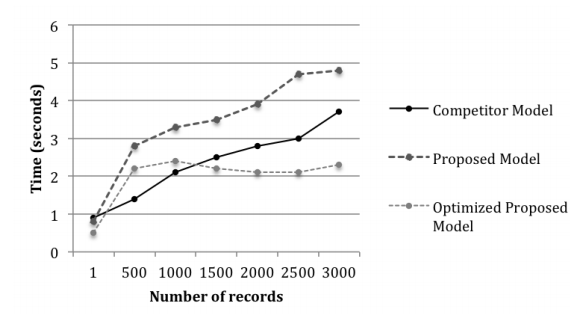
\includegraphics[height=6.2cm, width=\textwidth]{graph1.png}
     \caption{Time Spent in Synchronization client to Server(seconds)}\label{graph1}
     \end{figure}
     
     \begin{figure}[H]
     \centering
     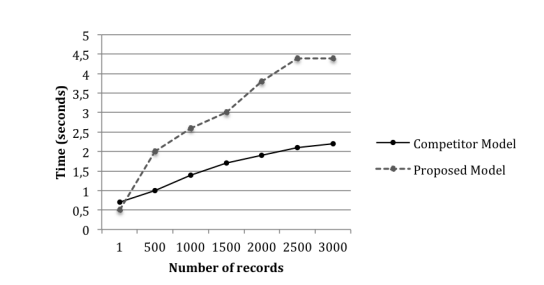
\includegraphics[height=6.2cm, width=\textwidth]{graph2.png}
      \caption{Time Spent in Synchronization Server to Client (seconds)}\label{graph2}
     \end{figure}
     
The first tests consisted of 500 successive records inserted into the client database. To each 500 records insertion, synchronization was performed and their times were measured. The second tests consisted of 500 consecutive insertion of records in the database server. As in the first test, at each insertion of 500 records, synchronization was performed and their times were measured. Comparing both the graphs, it can be concluded that the competitor model had lower times than the proposed model.

      
      \centering
      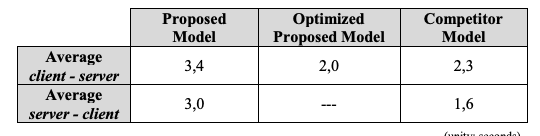
\includegraphics[height=5.2cm, width=\textwidth]{table1.png}
      \caption{Table 1: Average Time Synchronization between the models}
      
From Table 1 we can notice that the competitor model has lower times than the model proposed.So we can conclude, that most of the time spent was caused by the low efficiency of the Sync In algorithm implemented in the server’s side. 
}

\headerbox{Background}{name=background, column=1, span=2}
{Data synchronization between client devices and remote servers may happen through two distinct mechanisms: download and upload. The upload is performed first, thus corresponding to the transfer of data from the client application to a server, while the download corresponds to transferring data from the server to the client application. In both cases, the synchronization’s success or failure involves limitations at various levels, such as network availability and conflicts between different data. 

    \begin{figure}[H] 
    \centering
    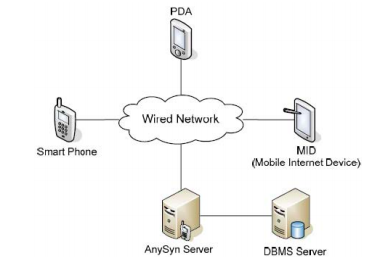
\includegraphics[height=7cm, width=9cm]{network.png}
    \caption{Typical Layout of Network Synchronization}\label{network}
    \end{figure}
    
In Figure 1. The server manages the database shared by all customers through the DBMS server. The client device’s user may construct the database client. 
}
\headerbox{Experiment}{name=experiment, column=2,span =1, below=background}
{The client application,synchronization agent implemented using Android platform in Java,the technology used for the RDBMS system was SQLite. The hash function MD5 was
used to produce the message digest. The synchronization agent was implemented using the PHP script, running on a web server.

Two types of tests were performed: synchronization tests after inserting records in the client’s side and synchronization tests after inserting records in the server’s side(shown in the Result section).
}

\headerbox{SAMD Algorithm}{name=SAMD Algorithm, column=1,span =1, below=background}
{
    \begin{figure}[H]
    \centering
    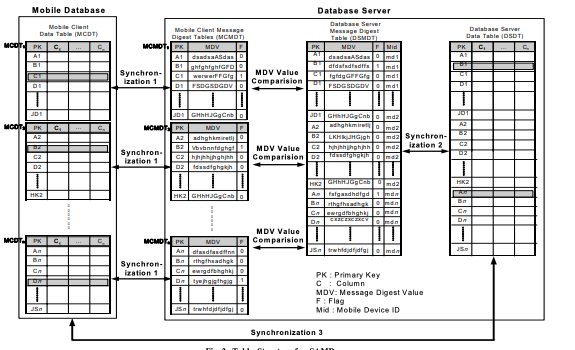
\includegraphics[height=9cm, width=9cm]{samd.png}
    \caption{Figure 2: Table Structure for SAMD}\label{samd}
    \end{figure}
    
Figure 4 displays the table schema of the server-side database
and the mobile database where the SAMD synchronization
algorithm is applied. 

The SAMD algorithm consists of synchronization 1,2 and 3 (Figure 4). 

Synchronizations 1 and 2 synchronize the data table and message digest table.Therefore, the two are identical synchronization algorithms applied to different tables. 

After SAMD algorithms analyze the type of inconsistency using the flag values, Synchronization 3 is performed between two data tables.

    \begin{figure}[H]
    \centering
    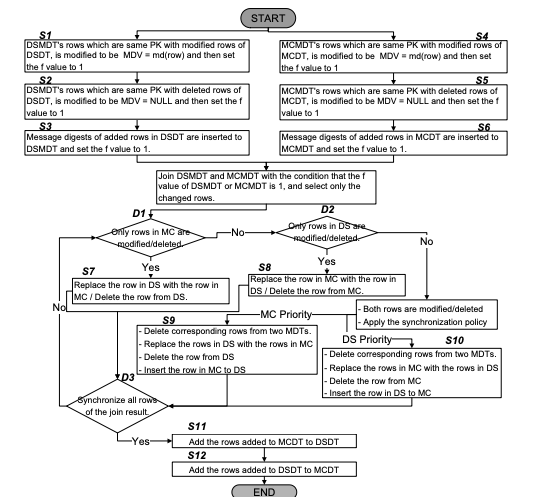
\includegraphics[height=9cm, width=9cm]{flowchart.png}
    \caption{SAMD Synchronization Algorithm}\label{flowchart}
    \end{figure}

Figure 5 exhibits the flow chart for the SAMD synchronization algorithm. 

Steps S1~S3 represent the Synchronization 2 stage of Figure 4.
Steps S4~S6 indicate the Synchronization 1 stage of Figure 4.
Steps S7~S12 display the Synchronization 3 stage of Figure 4.
}

\headerbox{Conclusion}{name=conclusion, column=2, span=1, below=experiment}
{The synchronization model minimizes the amount of data transmitted between the mobile device and the server, while reducing the processing in the device,leaving that processing to be done by the server.}

\headerbox{Future Work}{name=Future Work, column=2, span=1, below=conclusion}
{
 Given the growing number of businesses expanding to mobile environments, synchronization models like the one we proposed are important. In the future, the focus will continue to be the reduction of resources used by mobile devices. }

\headerbox{References}{name=references, column=2, span=1, below=Future Work}
{
\nocite{*}
\bibliographystyle{unsrt}
\bibliography{refer}


}
\end{poster}
\end{document}

